%%%%%%%%%%%%%%%%%%%%%%%%%%%%%%%%%%%%%%%%%
% Jacobs Landscape Poster
% LaTeX Template
% Version 1.1 (14/06/14)
%
% Created by:
% Computational Physics and Biophysics Group, Jacobs University
% https://teamwork.jacobs-university.de:8443/confluence/display/CoPandBiG/LaTeX+Poster
%
% Further modified by:
% Nathaniel Johnston (nathaniel@njohnston.ca)
%
% This template has been downloaded from:
% http://www.LaTeXTemplates.com
%
% License:
% CC BY-NC-SA 3.0 (http://creativecommons.org/licenses/by-nc-sa/3.0/)
%
%%%%%%%%%%%%%%%%%%%%%%%%%%%%%%%%%%%%%%%%%

%----------------------------------------------------------------------------------------
%	PACKAGES AND OTHER DOCUMENT CONFIGURATIONS
%----------------------------------------------------------------------------------------

\documentclass[final]{beamer}

\usepackage[scale=1.12]{beamerposter} % Use the beamerposter package for laying out the poster
\usepackage{listings}
\usepackage{fontspec}

\setmainfont{Georgia}

\usetheme{confposter} % Use the confposter theme supplied with this template

\setbeamercolor{block title}{fg=ngreen,bg=white} % Colors of the block titles
\setbeamercolor{block body}{fg=black,bg=white} % Colors of the body of blocks
\setbeamercolor{block alerted title}{fg=white,bg=dblue!70} % Colors of the highlighted block titles
\setbeamercolor{block alerted body}{fg=black,bg=dblue!10} % Colors of the body of highlighted blocks
% Many more colors are available for use in beamerthemeconfposter.sty

\setbeamerfont{block body}{series=\rmfamily}
%\setbeamerfont{block body}{series=\fontgeorgia}

%-----------------------------------------------------------
% Define the column widths and overall poster size
% To set effective sepwid, onecolwid and twocolwid values, first choose how many columns you want and how much separation you want between columns
% In this template, the separation width chosen is 0.024 of the paper width and a 4-column layout
% onecolwid should therefore be (1-(# of columns+1)*sepwid)/# of columns e.g. (1-(4+1)*0.024)/4 = 0.22
% Set twocolwid to be (2*onecolwid)+sepwid = 0.464
% Set threecolwid to be (3*onecolwid)+2*sepwid = 0.708

\newlength{\sepwid}
\newlength{\onecolwid}
\newlength{\twocolwid}
\newlength{\threecolwid}
\setlength{\paperwidth}{36in} % A0 width: 46.8in
\setlength{\paperheight}{36in} % A0 height: 33.1in
\setlength{\sepwid}{0.024\paperwidth} % Separation width (white space) between columns
\setlength{\onecolwid}{0.22\paperwidth} % Width of one column
\setlength{\twocolwid}{0.464\paperwidth} % Width of two columns
\setlength{\threecolwid}{0.708\paperwidth} % Width of three columns
\setlength{\topmargin}{-0.5in} % Reduce the top margin size
%-----------------------------------------------------------

\usepackage{graphicx}  % Required for including images

\usepackage{booktabs} % Top and bottom rules for tables

%----------------------------------------------------------------------------------------
%	TITLE SECTION
%----------------------------------------------------------------------------------------

\title{Efficient Parser and Pretty Printer Combinators in F2J} % Poster title

\author{Yuteng Zhong, Yi Li and Fan Xia} % Author(s)

\institute{Department of Computer Science, The University of Hong Kong} % Institution(s)

%----------------------------------------------------------------------------------------

\begin{document}

\addtobeamertemplate{block end}{}{\vspace*{2ex}} % White space under blocks
\addtobeamertemplate{block alerted end}{}{\vspace*{2ex}} % White space under highlighted (alert) blocks

\setlength{\belowcaptionskip}{1ex} % White space under figures
\setlength\belowdisplayshortskip{2ex} % White space under equations

\renewcommand{\raggedright}{\leftskip=0pt \rightskip=0pt plus 0cm}

\defverbatim[colored]\makeset{
\begin{lstlisting}


data PList[A]=Nil
|Cons A PList[A];
let rec recursive[A]
(a:A):A=recursive[A]
a;recursive[Int]1

data PList[A] = Nil | Cons A (PList[A]); let rec recursive[A] (a : A) : A = recursive[A] a; recursive[Int] 1

data PList[A]= 	Nil
            |   Cons A PList[A]
;
let rec recursive[A] (a: A): A =
    recursive[A] a
;
recursive[Int] 1

\end{lstlisting}
}


\begin{frame}[t] % The whole poster is enclosed in one beamer frame

\begin{columns}[t] % The whole poster consists of three major columns, the second of which is split into two columns twice - the [t] option aligns each column's content to the top

\begin{column}{\sepwid}\end{column} % Empty spacer column

\begin{column}{\onecolwid} % The first column

%----------------------------------------------------------------------------------------
%	The Tower of Babel
%----------------------------------------------------------------------------------------

\begin{figure}
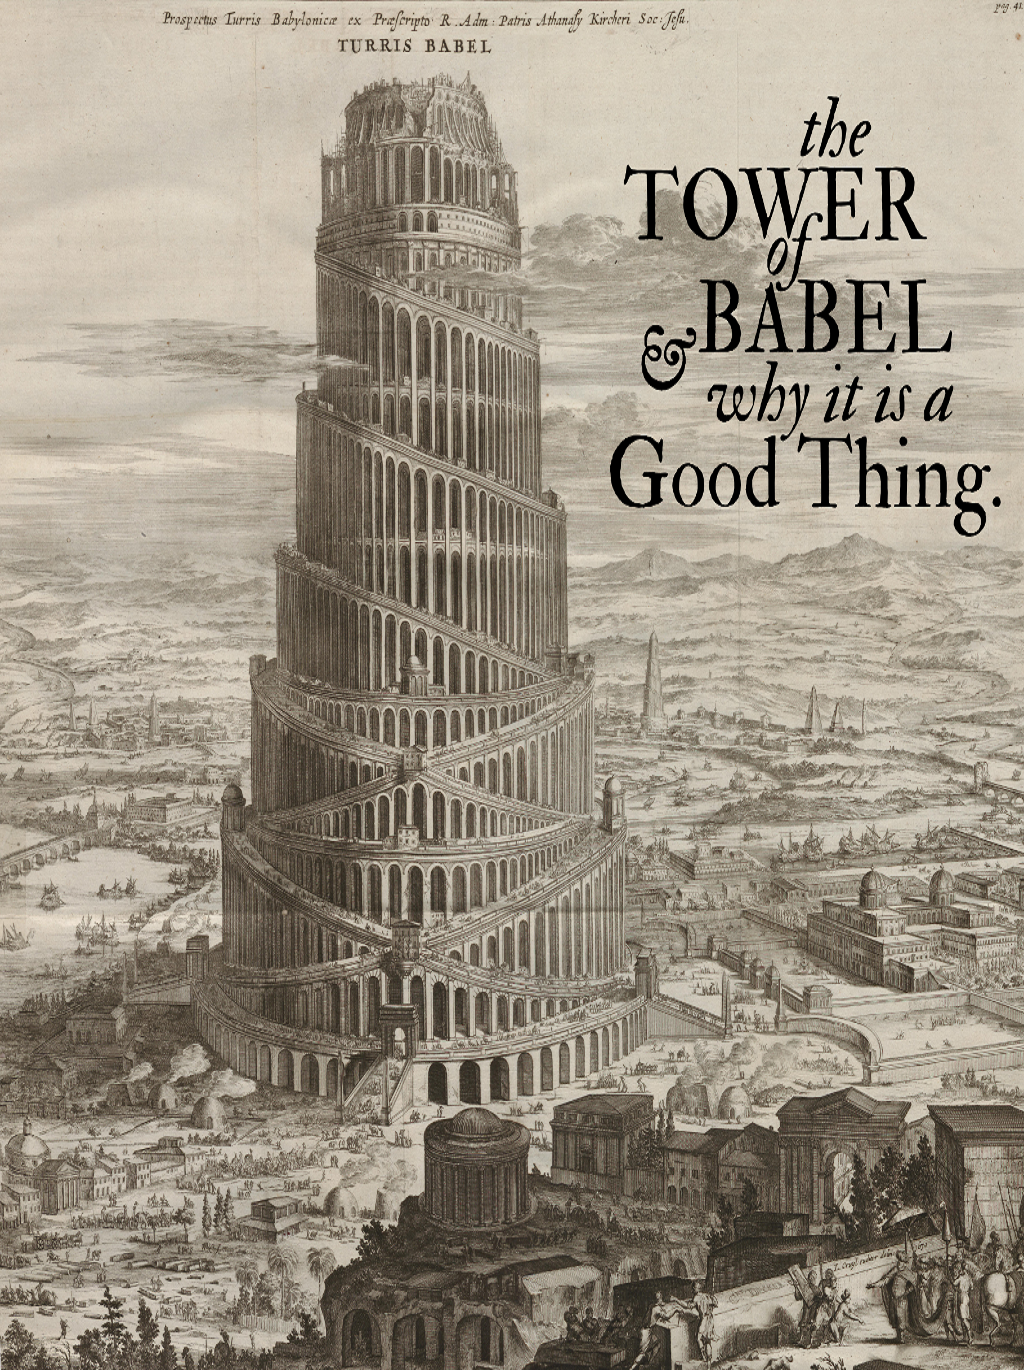
\includegraphics[width=\linewidth]{img/babellong.png}

\end{figure}

%----------------------------------------------------------------------------------------
%	MOTIVATION
%----------------------------------------------------------------------------------------

\begin{block}{Motivation}

At HKU, the Programming Languages group is developing a new JVM-based compiler for functional languages called F2J. 

\begin{figure}
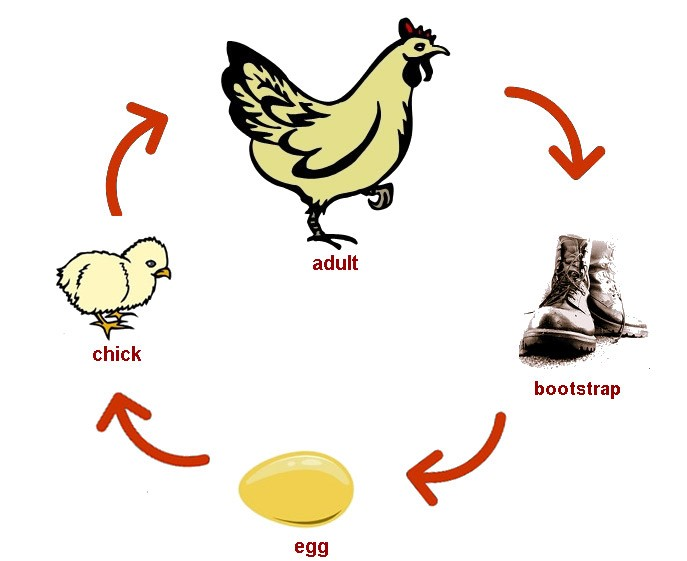
\includegraphics[width=0.9\linewidth]{img/bootstrapping.jpg}

\end{figure}

In order to make a selfhosting compiler, in other word, a \textbf{bootstrapped compiler} for F2J, we will need a parser. In this process, we could also build a pretty printer, which is a reversed process of parsing.

\end{block}

%----------------------------------------------------------------------------------------
%	INTRODUCTION
%----------------------------------------------------------------------------------------
\begin{block}{Introduction}

%A parser is a software component that takes input data and builds a data structure. Then pretty printer takes the data structure and generates designed output.

\textbf{Parsing and Printing:}

\begin{figure}
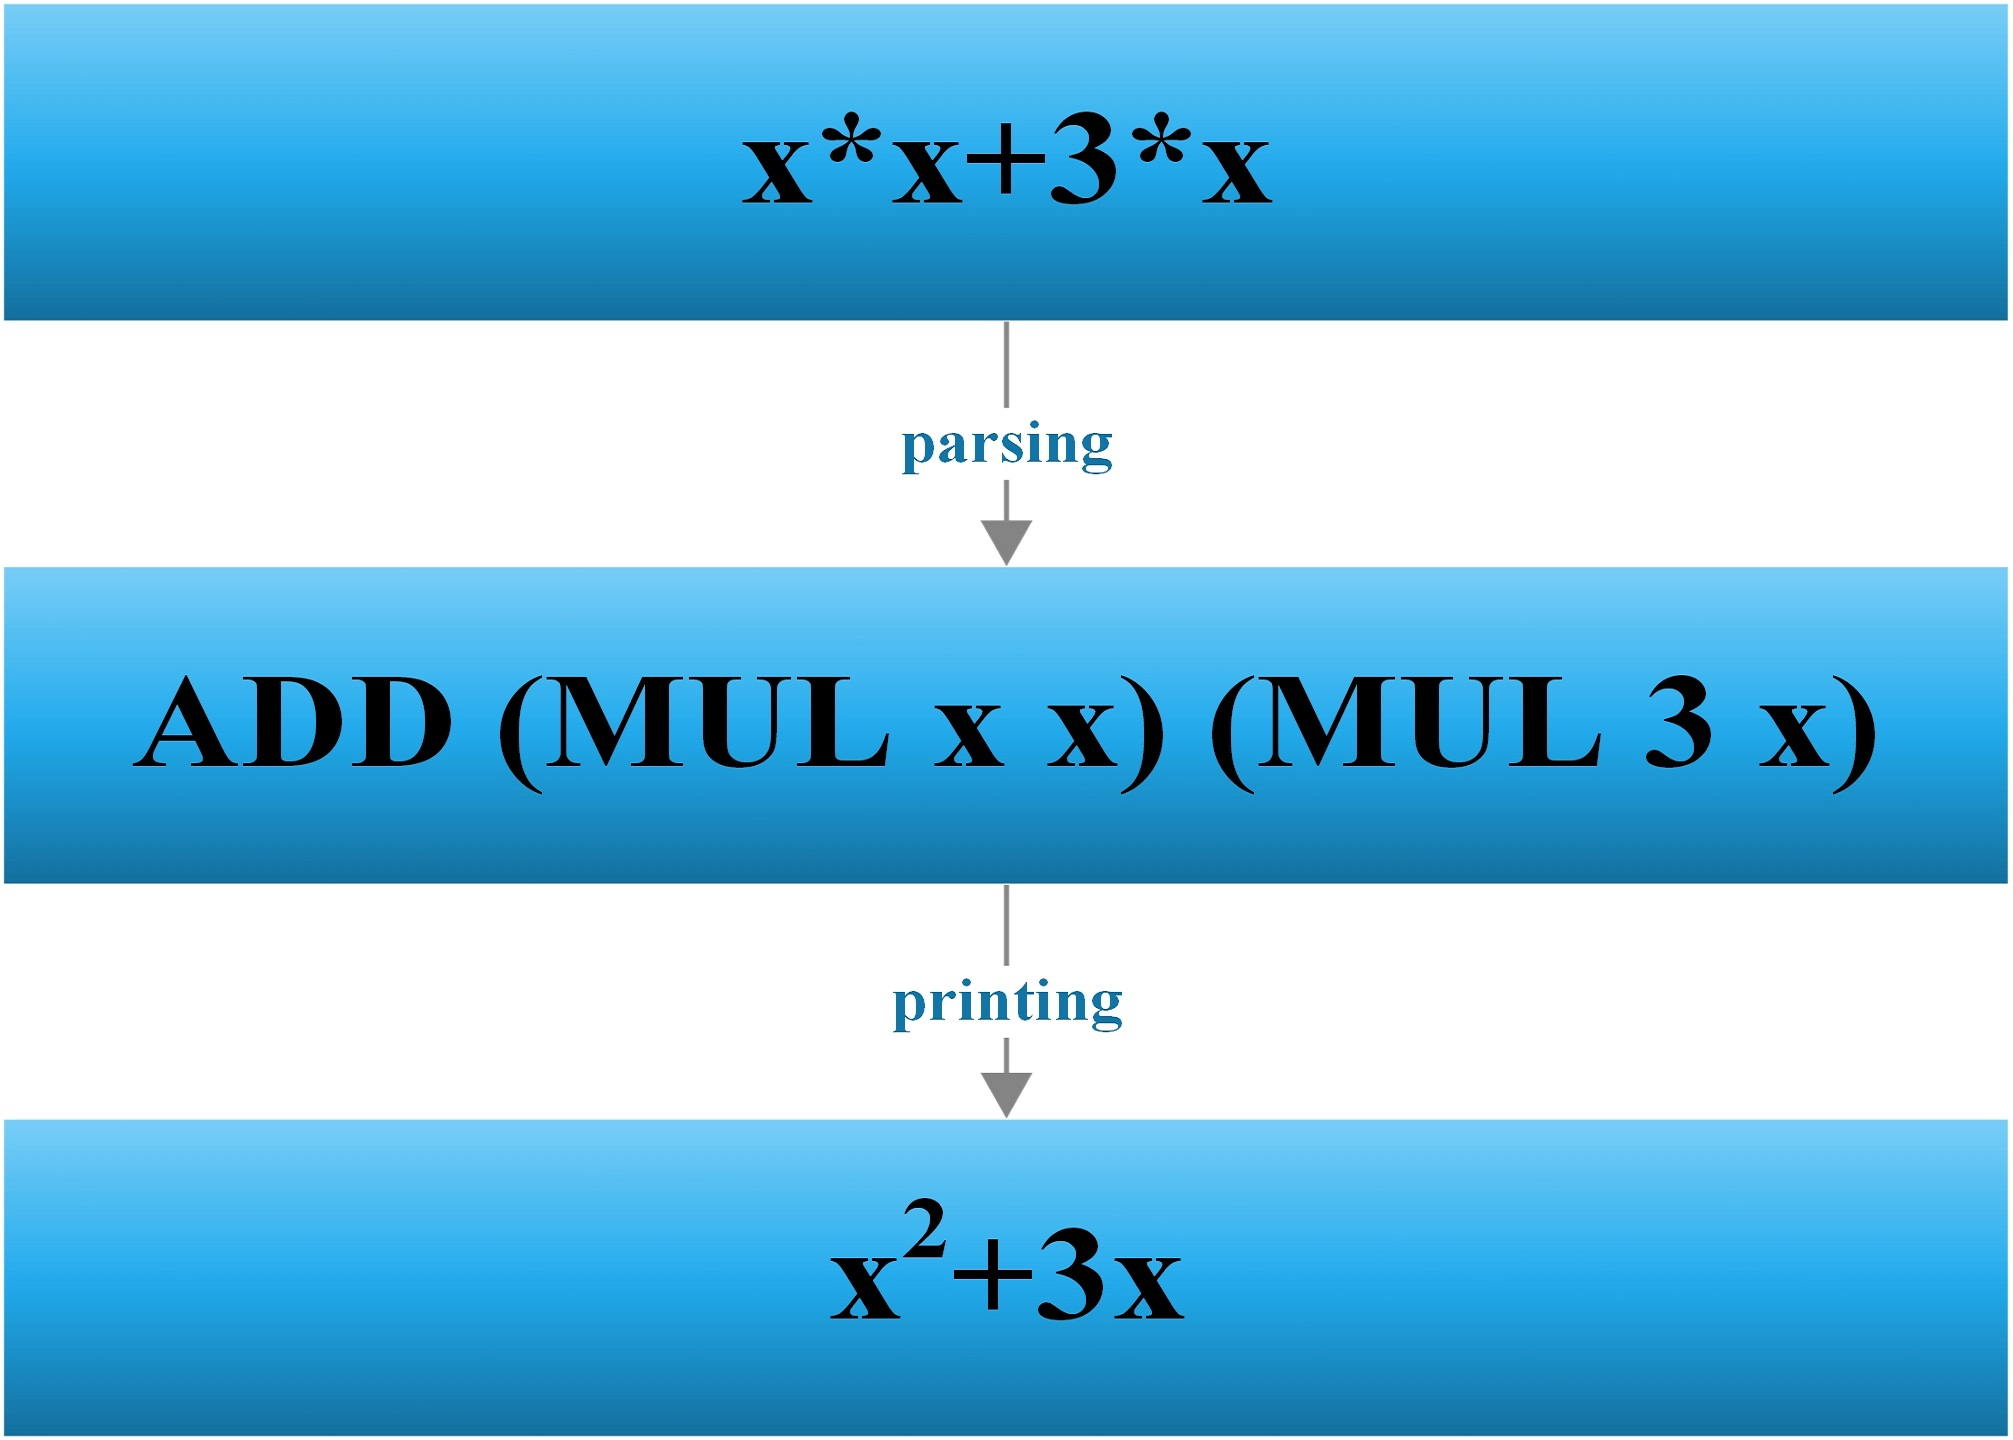
\includegraphics[width=0.75\linewidth]{img/parseprintershort.jpg}

\end{figure}


\end{block}


\end{column} % End of the first column

\begin{column}{\sepwid}\end{column} % Empty spacer column

\begin{column}{\twocolwid} % Begin a column which is two columns wide (column 2)

\begin{columns}[t,totalwidth=\twocolwid] % Split up the two columns wide column

\begin{column}{\onecolwid}\vspace{-.6in} % The first column within column 2 (column 2.1)

%----------------------------------------------------------------------------------------
%	MATERIALS
%----------------------------------------------------------------------------------------

\begin{block}{Introduction}

To parse a programming language, two common ways are used: \\
\textbf{Code generators:}
\begin{itemize}
\item flex
\item yacc
\end{itemize}
\textbf{Parser combinators:}
\begin{itemize}
\item planck in OCaml
\item parsec in Haskell
\end{itemize}

%Parser combinators are a set of higher-order functions that accepts several parser as input and then return a parser as output. In this context, a parser is a %function accepting strings as input and returning some structure as output, typically a parse tree or a set of indices representing locations in the string where %parsing stopped successfully. Parser combinators enable a recursive descent parsing strategy that facilitates modular piecewise construction and testing.
%This parsing technique is called combinatory parsing. Parser and Pretty Printer combinators are an alternative to tools used in compiler constructions, such as %lex, yacc or antlr. They have the advantage of being a library instead of a code generator tool.

\end{block}

%----------------------------------------------------------------------------------------

\end{column} % End of column 2.1

\begin{column}{\onecolwid}\vspace{-.6in} % The second column within column 2 (column 2.2)

%----------------------------------------------------------------------------------------
%	METHODS
%----------------------------------------------------------------------------------------

\begin{block}{Methods}

\textbf{Monadic:}

Monad is an algebraic structure from machematics that provided useful for addressing a
number of computational problems. Using a monadic sequencing combinator of parsers avoids
the messy manipulation of nested tuples of results present in early work. Moreover, using
monad comprehension notation makes parsers more compat and easy to read.

\textbf{Packrat:}

Packrat parsing provides the simplicity, elegance and generality of the backtracking model but eliminates the risk of super-linear parse time, by saving all intermediate parsing results as they are computed and ensuring that no result is evaluated more than once.

% The monad of parser can be expressed in a modular way in terms of two simpler monads. The
% immediate benefit is that the basic parser combinators no longer needs to be defined
% explicitly. Rather, they arise automatically as a special case of lifting monad operations
% from the base monad \textit{m} to a certain other monad parameterised over \textit{m}. This
% also means that, if we change the nature of parsers by modifying the base monad, then new
% combinators for the modified monad of parsers also arise automically via the lifting
% construction.


\end{block}

%----------------------------------------------------------------------------------------

\end{column} % End of column 2.2

\end{columns} % End of the split of column 2 - any content after this will now take up 2 columns width

%----------------------------------------------------------------------------------------
%	IMPORTANT RESULT
%----------------------------------------------------------------------------------------
\begin{alertblock}{MONAD}

\begin{figure}
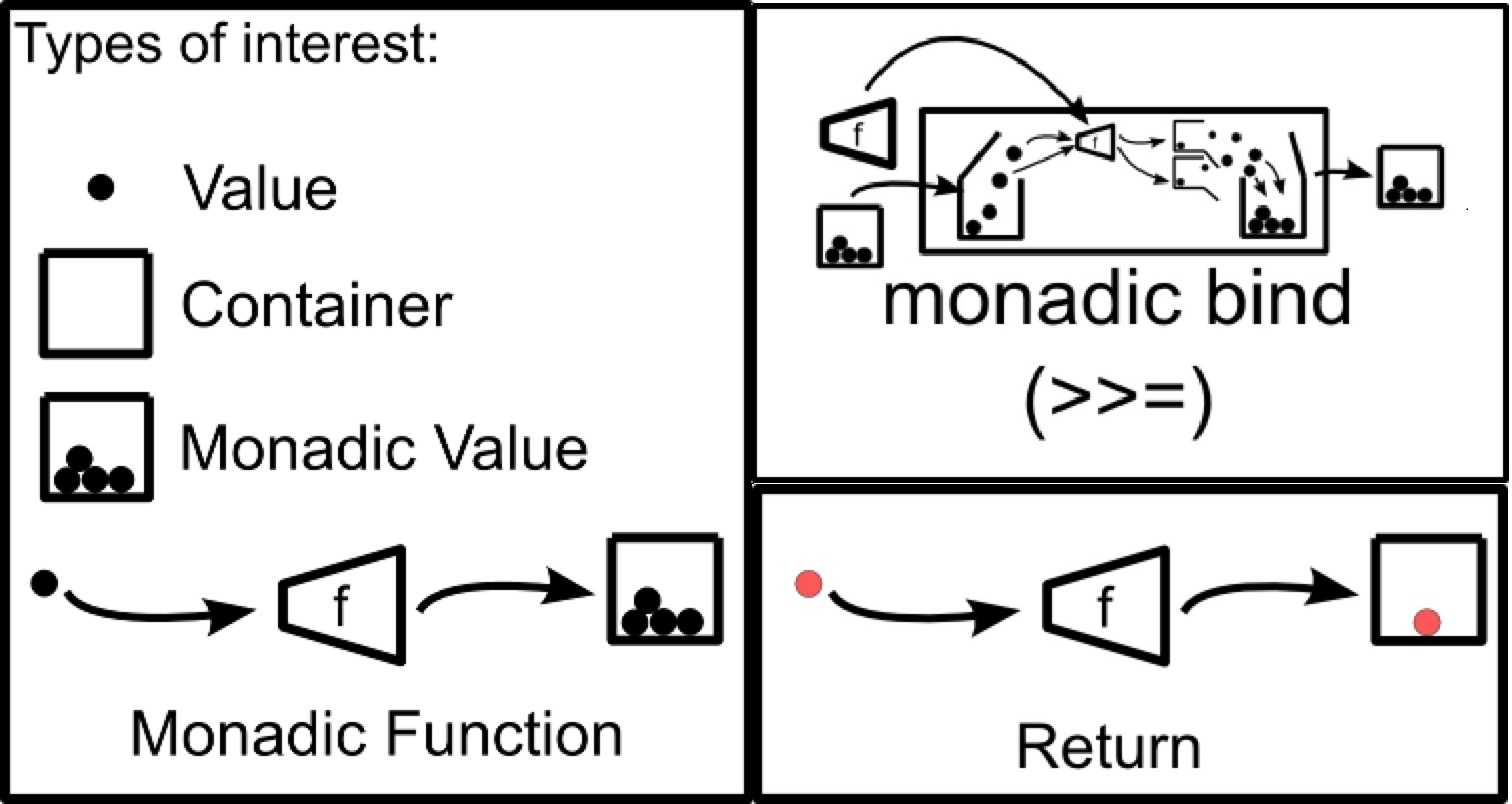
\includegraphics[width=0.8\linewidth]{img/monad.jpg}

\end{figure}
\end{alertblock}

%----------------------------------------------------------------------------------------

\begin{columns}[t,totalwidth=\twocolwid] % Split up the two columns wide column again

\begin{column}{\onecolwid} % The first column within column 2 (column 2.1)

%----------------------------------------------------------------------------------------
%	MATHEMATICAL SECTION
%----------------------------------------------------------------------------------------

\begin{block}{Optimisation}

\textbf{Parser}
\begin{itemize}
\item \textbf{Specific rules:} Try the most possible rules based on parsing context will help to find the correct result earlier.
%The parser will try the rules one by one.
\item \textbf{Lazy evaluation:} Parser combinators will generates all possible results in each level
of parse tree, lazy evaluation can enable the possibilty of ''parse by need''.
%, which will save lots of memory and time and become much more efficient.
\item \textbf{Reduce backtracking:} Backtracking is required when the parser encounter a failure.
% and then it may come back to the begining and try the other alternative rules.

\end{itemize}

\end{block}

%----------------------------------------------------------------------------------------

\end{column} % End of column 2.1

\begin{column}{\onecolwid} % The second column within column 2 (column 2.2)

%----------------------------------------------------------------------------------------
%	RESULTS
%----------------------------------------------------------------------------------------

\begin{block}{Optimisation}



\textbf{Pretty Printer}
\begin{itemize}
\item \textbf{Algebra:} Everything is based on a single concatenation operator that is associative.
\item \textbf{Optimality:} Optimal and Bounded. It means that the lib can choose line breaks to avoid overflow whenever possible, and it's done in O(n).
\item \textbf{Expressiveness:} Not as expressive as Hugh's library, but it is complete and enough for using.

\end{itemize}




%\begin{table}
%\vspace{2ex}
%\begin{tabular}{l l l}
%\toprule
%\textbf{Treatments} & \textbf{Response 1} & \textbf{Response 2}\\
%\midrule
%Treatment 1 & 0.0003262 & 0.562 \\
%Treatment 2 & 0.0015681 & 0.910 \\
%Treatment 3 & 0.0009271 & 0.296 \\
%\bottomrule
%\end{tabular}
%\caption{Table caption}
%\end{table}

\end{block}

%----------------------------------------------------------------------------------------

\end{column} % End of column 2.2

\end{columns} % End of the split of column 2

\end{column} % End of the second column

\begin{column}{\sepwid}\end{column} % Empty spacer column

\begin{column}{\onecolwid} % The third column


\begin{block}{Case Study}

\textbf{Parser and Pretty Printer for F2J}

\begin{figure}
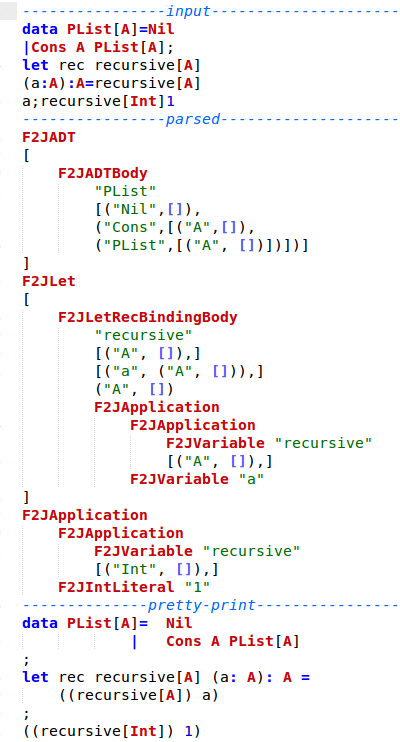
\includegraphics[width=\linewidth]{img/cs.jpg}

\end{figure}



\end{block}

%----------------------------------------------------------------------------------------
%	CONCLUSION
%----------------------------------------------------------------------------------------


\begin{block}{Conclusion}

 The greatest homage is imitation.


\end{block}



%----------------------------------------------------------------------------------------
%	ACKNOWLEDGEMENTS
%----------------------------------------------------------------------------------------

\setbeamercolor{block title}{fg=red,bg=white} % Change the block title color

\begin{block}{Acknowledgements}
\begin{itemize}
\item \small{\rmfamily{This project is under supervision of Dr.Bruno C. d. S. Oliveira and supportted by The University of Hong Kong Programming Languages Group.}}
\item \small{\rmfamily{Special thanks to Jeremy Bi, George Shi, Tomas, Emma, Ningning Xie, Linus Yang, Wexin Zhang and Yanlin.}} \\
\end{itemize}
\end{block}

%----------------------------------------------------------------------------------------
%	CONTACT INFORMATION
%----------------------------------------------------------------------------------------

%\setbeamercolor{block alerted title}{fg=black,bg=norange} % Change the alert block title colors
%\setbeamercolor{block alerted body}{fg=black,bg=white} % Change the alert block body colors

\begin{alertblock}{Contact Information}

\begin{itemize}
\item Web: https://github.com/hkuplg
\item Email: xiafan@hku.hk
\end{itemize}

\end{alertblock}

\begin{center}
\begin{tabular}{ccc}

\includegraphics[width=0.8\linewidth]{img/hkulogo} & \hfill &
\end{tabular}
\end{center}

%----------------------------------------------------------------------------------------

\end{column} % End of the third column

\end{columns} % End of all the columns in the poster

\end{frame} % End of the enclosing frame

\end{document}
